% !TeX program = xelatex
\documentclass[UTF8,12pt,a4paper,fontset=fandol]{ctexart}
\usepackage[top=23mm,bottom=24mm,left=24mm,right=24mm]{geometry}
\usepackage{amsmath,amssymb,amsthm,booktabs,tikz}
\usepackage[unicode,hidelinks]{hyperref}
\hypersetup{pdftitle={哪些窗口长度足以判定圆环布点均衡？}}
\ctexset{section={format=\large\bfseries,beforeskip=1.0ex,afterskip=.65ex}}
\newtheoremstyle{plaincn}{.65em}{.45em}{\normalfont}{}{\bfseries}{\quad}{0pt}{}
\theoremstyle{plaincn}
\newtheorem{theorem}{定理}
\newtheorem{lemma}[theorem]{引理}
\newtheorem{corollary}[theorem]{推论}
\renewcommand{\proofname}{证明}
\linespread{1.22}
\setlength{\parskip}{.35em}
\newcommand{\fl}[1]{\left\lfloor #1\right\rfloor}
\newcommand{\cl}[1]{\left\lceil #1\right\rceil}
\newcommand{\Z}{\mathbb Z}
\newcommand{\E}{\mathbb E}
\newcommand{\Prob}{\mathbb P}
\newcommand{\nextsec}[1]{\clearpage\section{#1}}
\begin{document}
\begin{center}
{\LARGE\bfseries 哪些窗口长度足以判定圆环布点均衡？\par}
\vspace{.4em}
{\large 循环二元词的判定与相关失效下的首次探测\par}
\end{center}

\noindent\textbf{摘要}\quad
在 $N$ 个格点的圆环上标记 $m$ 个点。若任意两个等长窗口所含标记数相差至多一，称布置均衡。给定一组窗口长度，本文给出该组测试足以推出所有长度均衡的充要条件。最少测试长度数恰为零、一或二，并可由 $m/N$ 的既约分数直接读出。必要性证明构造了能通过全部指定测试的非均衡布置。作为应用，若按环序编号的探测点具有循环平移不变的联合失效分布，均衡布置同时极小化任意均匀起点近邻游走在每个截止时刻的漏检概率。文中给出精确最优值，并说明何时独立失效下的少数窗口足以辨认所有通用最优布置。

\section{两个相同的间距表，为何有不同的漏检概率？}
在十个格点上放四个探测点。下图中的两种布置都有两个长度为 $2$ 和两个长度为 $3$ 的间距。取均匀随机起点，顺时针查看含起点在内的五格。布置 A 的每个窗口恰含两点。布置 B 则有一个窗口含一点、一个含三点，另八个都含两点。
\begin{center}
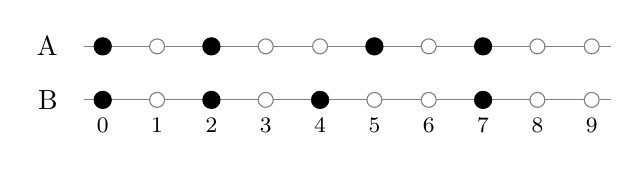
\begin{tikzpicture}[x=.69cm,y=.68cm]
\foreach \y/\lab in {1/A,0/B}{
 \node[left] at (-.65,\y) {\lab};
 \draw[gray] (-.35,\y)--(9.35,\y);
 \foreach \x in {0,...,9} {\filldraw[fill=white,draw=gray] (\x,\y) circle (2.7pt);}
}
\foreach \x in {0,2,5,7} {\fill (\x,1) circle (3.3pt);}
\foreach \x in {0,2,4,7} {\fill (\x,0) circle (3.3pt);}
\foreach \x in {0,...,9} {\node[below,font=\footnotesize] at (\x,-.16) {\x};}
\end{tikzpicture}

{\small 图 1\quad 将圆环在格点 $0$ 展开。实心点是探测点，格点 $9$ 与 $0$ 相邻。}
\end{center}
若各点独立地以概率 $1/2$ 失效，A 的漏检概率为 $1/4$，B 为
$(2^{-1}+8\cdot2^{-2}+2^{-3})/10=21/80$。差别来自间距的排列顺序。要确认一个布置对所有窗口都最优，究竟需要检查多少种长度？

设 $0<m<N$，用 $N$ 周期的二元序列 $a=(a_x)$ 表示布置，一周期内有 $m$ 个 $1$。定义
\[
 C_\ell(x)=\sum_{j=0}^{\ell-1}a_{x+j},\qquad
 W_\ell:\quad \max_x C_\ell(x)-\min_x C_\ell(x)\le1 .
\]
每一点被恰好 $\ell$ 个窗口覆盖，所以 $C_\ell$ 的均值等于 $m\ell/N$。条件 $W_\ell$ 等价于每个计数都取该均值的下整或上整。满足所有 $W_\ell$ 的词称为\textbf{循环均衡词}。经典构造为
\begin{equation}
 b_x=\fl{(x+1)m/N}-\fl{xm/N}.                          \label{eq:word}
\end{equation}
其窗口和可望远镜相消，故各长度均衡。固定长度与重量时，均衡词构成一个旋转轨道，见 Wu \cite{wu}。下文同时给出这一事实的直接证明。

\nextsec{一组窗口长度何时足够}
称 $L\subseteq\{1,\ldots,N-1\}$ 为\textbf{判定集}，若每个通过全部 $\ell\in L$ 测试的重量 $m$ 循环词都均衡。每个长度的测试都覆盖全部起点。记
\[
 d=\gcd(N,m),\qquad n=N/d,\qquad h=m/d,\qquad
 G=\gcd\bigl(\{N\}\cup\{\ell\in L:n\mid\ell\}\bigr).
\]
于是 $m/N=h/n$ 且 $\gcd(h,n)=1$。若没有 $n$ 的倍数入选，则 $G=N$。

\begin{theorem}[窗口长度判据]\label{thm:main}
$L$ 为判定集当且仅当以下两条同时成立：
\begin{align}
 &G=n, \label{eq:period}\\
 &\min(h,n-h)=1\quad\text{或存在 }\ell\in L\text{ 使 }h\ell\equiv 1
       \text{ 或 }-1\pmod n . \label{eq:shape}
\end{align}
\end{theorem}

\noindent\textbf{充分性。}
若 $n\mid\ell$，则均值 $h\ell/n$ 为整数，通过 $W_\ell$ 即说明所有窗口和相等。相邻窗口相减给出
\begin{equation}
 C_\ell(x+1)-C_\ell(x)=a_{x+\ell}-a_x .                 \label{eq:diff}
\end{equation}
故 $\ell$ 是 $a$ 的一个周期。序列已有周期 $N$，其整数周期构成加法子群，因此 $G$ 也是周期。条件 \eqref{eq:period} 把问题化为长度 $n$、重量 $h$ 的一周期。如果 $h=1$ 或 $n-h=1$，单个 $1$ 或单个 $0$ 的位置已将周期词确定到旋转。

余设 \eqref{eq:shape} 中的同余成立。将 $\ell$ 对 $n$ 取余得 $s$，去掉整周期只会给各窗口和减去同一常数。若 $hs\equiv-1$，改测 $n-s$ 即可，因为互补窗口的和为 $h$。故只需考虑 $hs\equiv1\pmod n$。令 $j=(hs-1)/n$。均衡的 $n$ 个长度 $s$ 窗口和之总和为 $hs=nj+1$，于是恰好一个起点取 $j+1$，其余都取 $j$。将待判定词旋转，使这一特殊起点与式 \eqref{eq:word} 的特殊起点重合。两词的长度 $s$ 窗口和逐项相同。由式 \eqref{eq:diff}，两词之差以 $s$ 为周期，又以 $n$ 为周期。由于 $\gcd(s,n)=1$，该差为常数。两词重量相同，故常数为零。这就证明了充分性，也证明所有均衡词都是式 \eqref{eq:word} 的旋转。后者可取 $L$ 为全部长度应用以上论证。

\begin{corollary}[恰好需要几种长度]\label{cor:number}
最小判定集的大小等于
\[
 \boldsymbol{1}_{d>1}+\boldsymbol{1}_{\min(h,n-h)>1}.
\]
第一项非零时可选 $\ell=n$，第二项非零时可选 $h$ 模 $n$ 的乘法逆元在 $1,\ldots,n-1$ 中的代表。
\end{corollary}
\noindent 由定理，$d>1$ 时至少需要一个 $n$ 的倍数，第二项非零时还需要一个不被 $n$ 整除的长度。这两种长度各有独立作用。例如 $N=10,m=4$ 时，$n=5,h=2$，可选 $5$ 和 $2$，因为 $2\cdot2\equiv-1\pmod5$。只检验一种长度，无论怎样选都不能完成判定。

\nextsec{必要性：能躲过指定长度的两个构造}
设 $F(x)=\fl{hx/n}$，相位 $r_x$ 是 $hx$ 模 $n$ 在 $0,\ldots,n-1$ 中的代表。取 $N$ 周期的 $\{0,1\}$ 值函数 $u(x)$，令 $H=F+u$，候选词为 $a_x=H(x+1)-H(x)$。其一周期增量为 $m$。检验窗长 $\ell$ 时只需考察 $H(x+\ell)-H(x)$。

\begin{lemma}[抬高某一相位]\label{lem:raise}
仅在相位为 $z$ 的某些位置将 $F$ 加一。记 $R=h\ell\bmod n$。若 $R=0$ 且 $u$ 以 $\ell$ 为周期，则窗长 $\ell$ 的计数不变。若 $R>0$ 且 $z\ge\max(R,n-R)$，则抬高后仍然通过长度 $\ell$ 的下整、上整测试。
\end{lemma}
\begin{proof}
原窗口和是 $\fl{h\ell/n}$ 加上进位 $\boldsymbol{1}_{r_x+R\ge n}$。在 $R>0$ 时两端相位不同，至多一端被抬高。若起点被抬高，其相位 $z\ge n-R$ 保证原有进位，窗口和减一后恰取下整。若终点被抬高，由 $z\ge R$ 知起点相位为 $z-R$，原无进位，窗口和加一后恰取上整。两端都不动时结论直接成立。$R=0$ 的情形由端点改变量相等得到。
\end{proof}

\noindent\textbf{缺少周期条件。}
若 $G>n$，则 $n\mid G\mid N$。取 $r_y=n-1$ 的一个 $y$，恰在 $x\equiv y\pmod G$ 的位置抬高。这些位置相位均为 $n-1$。对 $L$ 中每个 $n$ 的倍数，$G\mid\ell$，故两个端点的改变量相同。对其余长度，引理对 $z=n-1$ 适用。长度 $1$ 也满足引理，所以新序列确实是一个二元词。它却不通过 $W_n$：从 $y$ 到 $y+n$ 的窗口和为 $h-1$，而所有长度 $n$ 的窗口均值为 $h$。这给出了能同时躲过 $L$ 全部测试的反例。

\noindent\textbf{缺少形状条件。}
此时 $2\le h\le n-2$，且 $L$ 中每个非零余数 $R$ 都属于 $[2,n-2]$。恰在相位 $z=n-2$ 的所有位置抬高。$u$ 是 $n$ 周期的，因此所有整数均值的长度均通过测试。其余入选长度都满足 $z\ge\max(R,n-R)$。长度 $1$ 的余数为 $h$，也在同一范围，故构造仍为二元词。

取 $s\in\{1,\ldots,n-1\}$ 使 $hs\equiv1\pmod n$。从相位 $n-2$ 出发，走 $s$ 格后相位为 $n-1$。原窗口没有进位，新的窗口仅起点抬高，和变为 $\fl{hs/n}-1$，低于许可范围。于是 $W_s$ 失败。两个构造分别证明了定理 \ref{thm:main} 的两条必要条件。\hfill$\square$

\medskip
\noindent\textbf{判定的代价。}
给定一段实际的二元数据，首个窗口求和后，用式 \eqref{eq:diff} 每移动一格只做一次加、减。用推论 \ref{cor:number} 选定长度，至多扫描两遍即可判定全局均衡，除输入外只需常数个机器字。这里的最少性针对所检查的\emph{长度种数}，每种长度仍须按定义检查其全部起点。

\nextsec{相关失效下，每个探测截止时刻的精确最优值}
给 $m$ 个探测点按顺时针编号。一次实验开始时抽取并固定它们的有效或失效状态。假设该向量的联合分布对编号的循环平移不变，且比较不同布置时使用同一个编号分布。相邻多点一起失效、恰有给定数目的点有效、独立失效都符合这一假设。记 $D_i$ 为编号 $i$ 失效的事件，下标按模 $m$ 计算，并令
\[
 q(0)=1,\qquad q(k)=\Prob(D_1\cap\cdots\cap D_k),\quad 1\le k\le m .
\]
均匀随机的长度 $\ell$ 窗口漏检的概率记为 $V_a(\ell)$。窗口起点与状态独立，漏检指窗口内没有有效探测点。

\begin{theorem}[最优漏检概率]\label{thm:void}
设 $\widetilde q$ 是 $q(0),\ldots,q(m)$ 间的分段线性插值。则对 $1\le\ell\le N$，
\begin{equation}
 V_a(\ell)=\frac1N\sum_{x=0}^{N-1}q(C_\ell(x))
 \ \ge\ \widetilde q(m\ell/N)=V_b(\ell).                \label{eq:void}
\end{equation}
若每个点独立地以同一概率 $p\in(0,1)$ 失效，则对指定 $\ell$，等号成立当且仅当 $W_\ell$ 成立。
\end{theorem}
\begin{proof}
窗口中的点按编号形成连续块。由循环不变性，其全体失效概率只依赖块长，故得等式左端。再看相邻斜率，对于 $1\le k<m$，平移不变性给出
\[
 q(k-1)-2q(k)+q(k+1)
 =\Prob\!\left(D_0^{\,c}\cap D_1\cap\cdots\cap D_{k-1}\cap D_k^{\,c}\right)\ge0 .
\]
当 $k=1$ 时中间的交为空条件。这个恒等式只用两次容斥，因而允许相关失效。$\widetilde q$ 凸，代入窗口计数的均值即可用 Jensen 不等式得到下界。式 \eqref{eq:word} 的所有窗口值都在均值两侧的相邻整数上，插值使下界取等。独立时 $q(k)=p^k$，相邻差分严格递增。若最大与最小计数相差至少二，使其各向中间移一格便会严格降低两项之和，反复平衡可达相邻整数分布。故原值严格大于下界。
\end{proof}

\noindent\textbf{首次探测。}
令 $X_t=U+Y_t\bmod N$，其中 $U$ 在圆环上均匀，$Y_0=0$ 且 $Y_{t+1}-Y_t\in\{-1,0,1\}$。起点 $U$、相对路径 $(Y_t)$、探测点状态三者独立。路径可以确定，也可有偏或有记忆。令 $T_a$ 为首次访问有效点的时刻，起点也算访问，未探测时取 $+\infty$。给定截至 $t$ 的相对路径，访问集合是某个连续窗口的均匀平移，其大小为
\[
 R_t=\min\{N,\ 1+\max_{0\le j\le t}Y_j-\min_{0\le j\le t}Y_j\}.
\]
因此 $\Prob(T_a>t)=\E[V_a(R_t)]\ge\E[\widetilde q(mR_t/N)]=\Prob(T_b>t)$。同一布置同时达到每个时刻的最小尾概率，且最小化每个截断期望 $\E[\min(T_a,H)]$。容许全体失效时，无条件期望可能为无穷，尾概率和截断期望仍有意义。

\nextsec{如何辨认通用最优布置}
设只用一种独立失效概率 $p\in(0,1)$ 做标准比较。对每个指定长度 $\ell$，取顺时针单位步长的路径，在 $t=\ell-1$ 时比较漏检概率。此时路径恰访问 $\ell$ 格。由定理 \ref{thm:void} 的严格取等条件，达到理论最优值等价于通过 $W_\ell$。因此得到一个跨失效模型的推论。

\begin{corollary}\label{cor:universal}
对于固定 $N,m$，上述标准比较在 $L$ 上全部取等足以保证布置对\emph{每种}循环平移不变的失效分布、\emph{每条}满足假设的近邻路径及\emph{每个}截止时刻都最优，当且仅当 $L$ 满足定理 \ref{thm:main}。此处比较的是精确概率。
\end{corollary}
\begin{proof}
条件成立时该布置均衡，应用式 \eqref{eq:void} 即得结论。条件失败时，第 3 节构造的反例通过所有指定长度，却在另一长度 $s$ 不均衡。保持同一个 $p$，取顺时针路径并在 $s-1$ 截止，漏检概率严格较高。
\end{proof}

\noindent\textbf{两项边界。}
若恰有一个均匀随机编号的点有效，则 $q(k)=1-k/m$，对所有布置都有 $V_a(\ell)=1-\ell/N$。因此相关失效下最优布置可能增多。若路径可以跨格跳跃，结论本身也可能失效。取 $N=4,m=2$，各点均有效，访问 $U,U+2$ 两格。均衡布置 $\{0,2\}$ 的漏检概率为 $1/2$，布置 $\{0,1\}$ 的漏检概率为零。这正是访问集不再构成连续窗口的情形。

\noindent\textbf{与前作的关系。}
Wu 讨论规则圆环配置的构造、唯一性及其与均衡词的关系 \cite{wu}。Lin 的周界巡逻模型中，独立探测时让通过次数集中于均值两侧相邻整数的论证，已见其引理 1 \cite{lin}。Frasca 等讨论连续圆周上到最近有效传感器的最大距离，证明独立失效下等距布点最小化这一距离的期望 \cite[命题 5]{frasca}。本文处理固定离散格点上的窗口长度判定集，以及按环序相关失效时首次探测时间的尾概率。以上比较限于所引文献，定理的证明不依赖首发性判断。

\noindent\textbf{有限核验。}
附带程序使用 Python 标准库。对 $2\le N\le12$，按定义枚举 $8\,166$ 个非常值有标号布置，再对 $40\,962$ 个 $(N,m,L)$ 比较定理 \ref{thm:main} 的双向预测。对 $N\le8$，遍历每个二元失效向量及其循环平移，逐起点直接计算漏检，共核对 $70\,190$ 个布置、失效向量和窗长组合。两项检查均使用整数计数，全部通过。任意循环不变的失效分布都是这些均匀轨道分布的混合。

{\small
\begin{thebibliography}{9}\setlength{\itemsep}{.12em}
\bibitem{wu} T. Wu. \href{https://arxiv.org/abs/0710.0125}{On regular configurations and disjoint cycles in shift graphs}. arXiv:0710.0125, 2007.
\bibitem{lin} K. Y. Lin. \href{https://doi.org/10.1287/opre.2021.2117}{Technical Note—Optimal Patrol of a Perimeter}. \emph{Operations Research} 70(5), 2860--2866, 2022.
\bibitem{frasca} P. Frasca, F. Garin, B. Gerencsér, J. M. Hendrickx. \href{https://doi.org/10.1137/140968094}{Optimal One-Dimensional Coverage by Unreliable Sensors}. \emph{SIAM J. Control Optim.} 53(5), 3120--3140, 2015.
\end{thebibliography}}
\end{document}
